% !TeX root = ../main.tex

\section{Tool Demonstration}

This section provides a practical demonstration of \tool{} through concrete examples showing how the framework handles different aspects of Java-to-C++ translation.

\subsection{Example: Cookie Class Translation}

We demonstrate the translation process using a simplified Cookie class, which illustrates the hierarchical approach and error resolution capabilities.

\subsubsection{Original Java Code}

\begin{figure}[h]
\centering
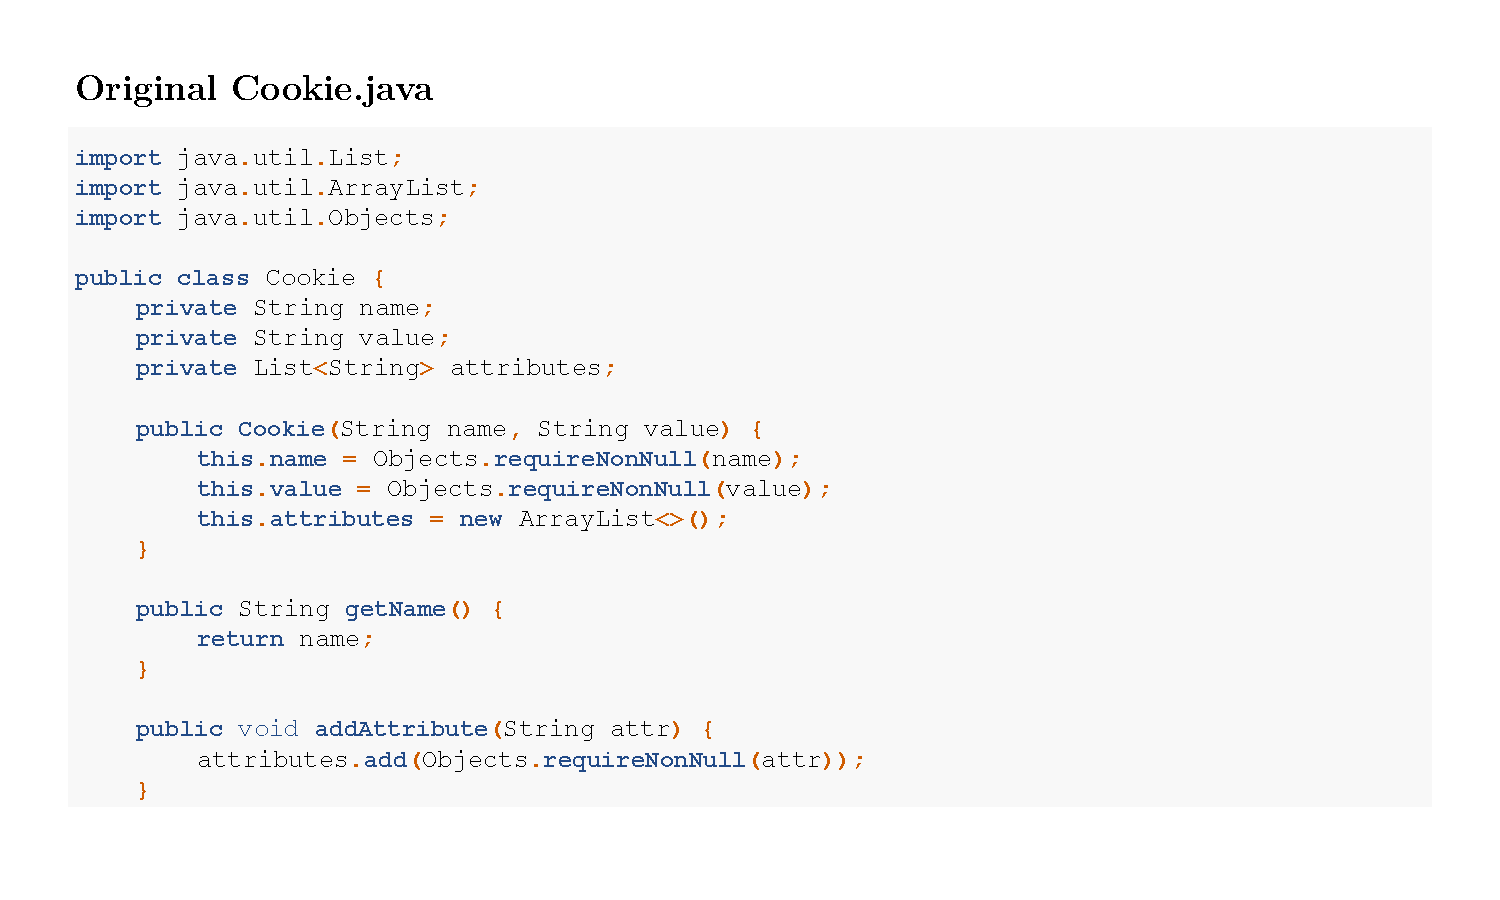
\includegraphics[width=\columnwidth]{code/fig5-1-cookie-original-java.pdf}
\caption{Original Cookie.java}
\label{fig:original-java}
\end{figure}

\subsubsection{Phase 1: Class-Level Translation Scheme}

The LLM generates a high-level translation strategy:

\begin{figure}[h]
\centering
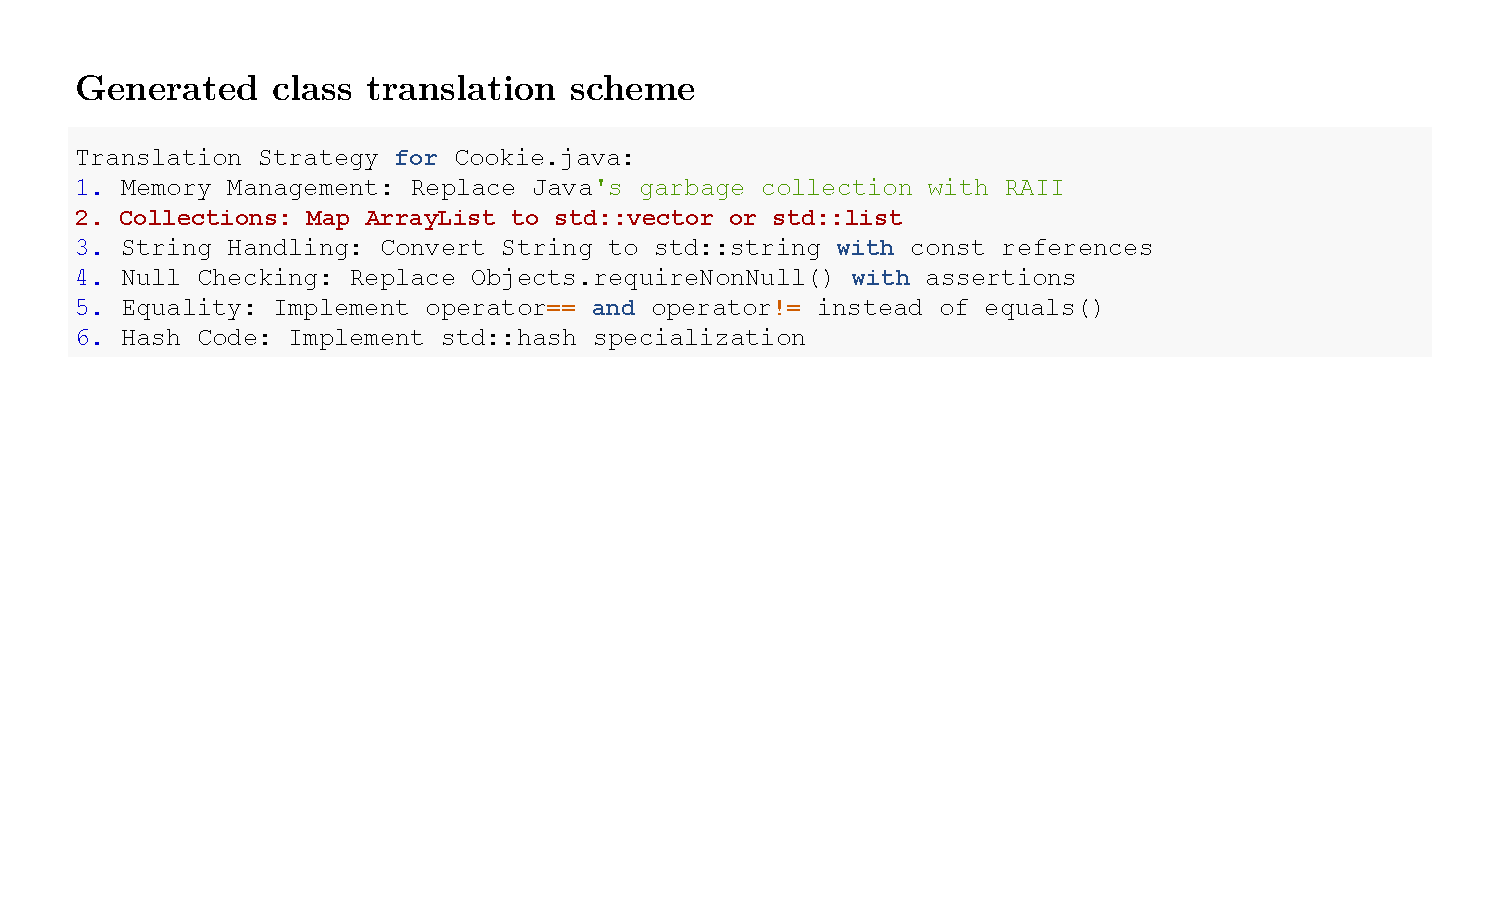
\includegraphics[width=\columnwidth]{code/fig5-2-cookie-translation-scheme.pdf}
\caption{Generated class translation scheme}
\label{fig:translation-scheme}
\end{figure}

\subsubsection{Phase 2: Method-Level Translation}

Based on the call graph analysis, methods are translated in dependency order:

\begin{figure}[h]
\centering
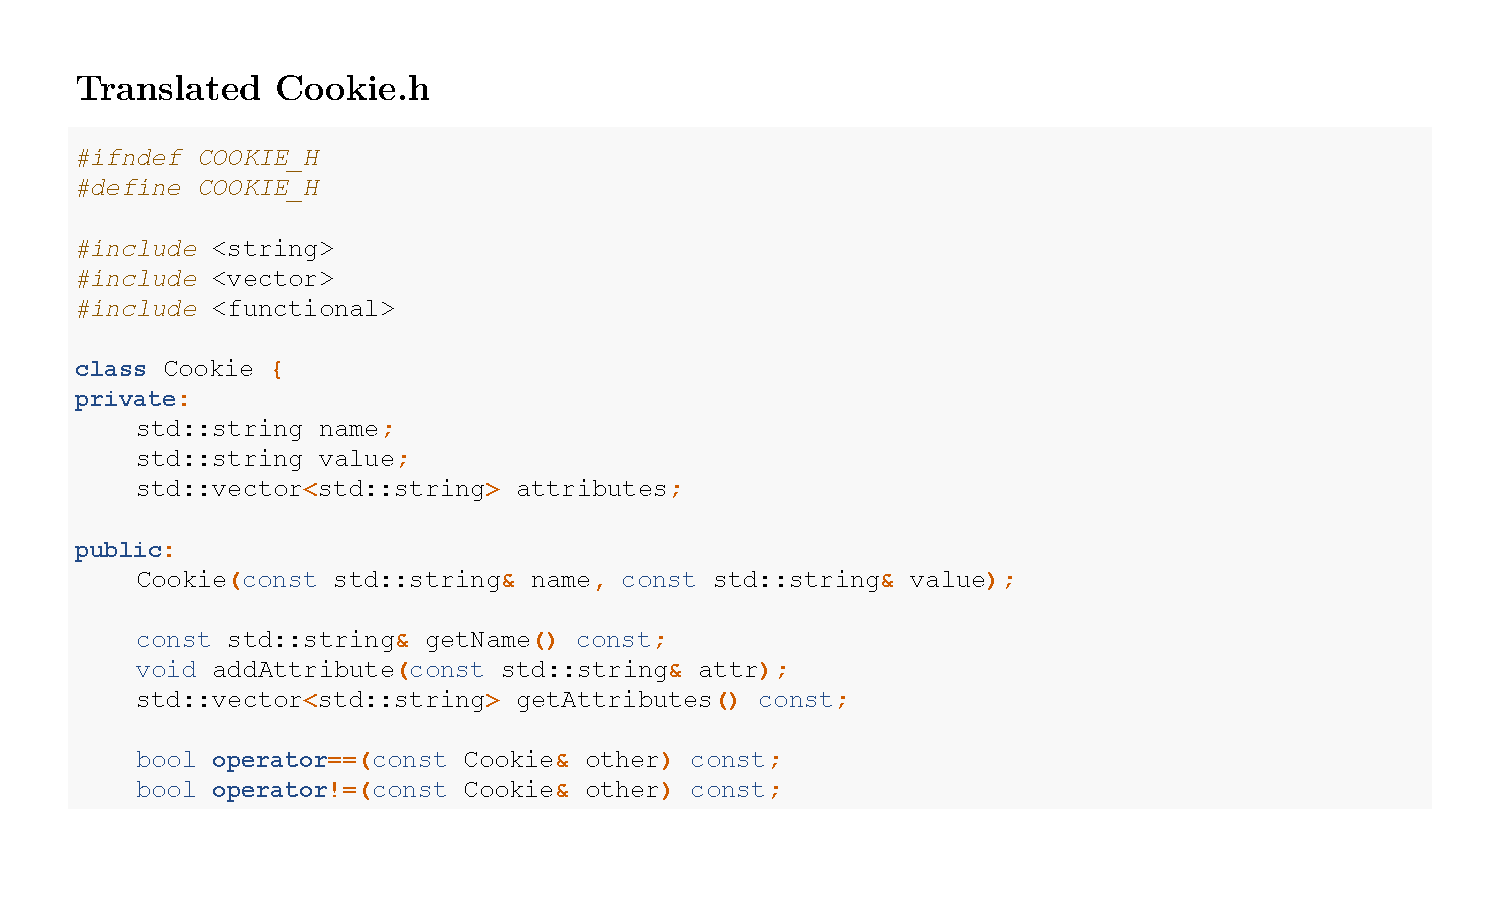
\includegraphics[width=\columnwidth]{code/fig5-3-cookie-translated-h.pdf}
\caption{Translated Cookie.h}
\label{fig:cpp-header}
\end{figure}

\begin{figure}[h]
\centering
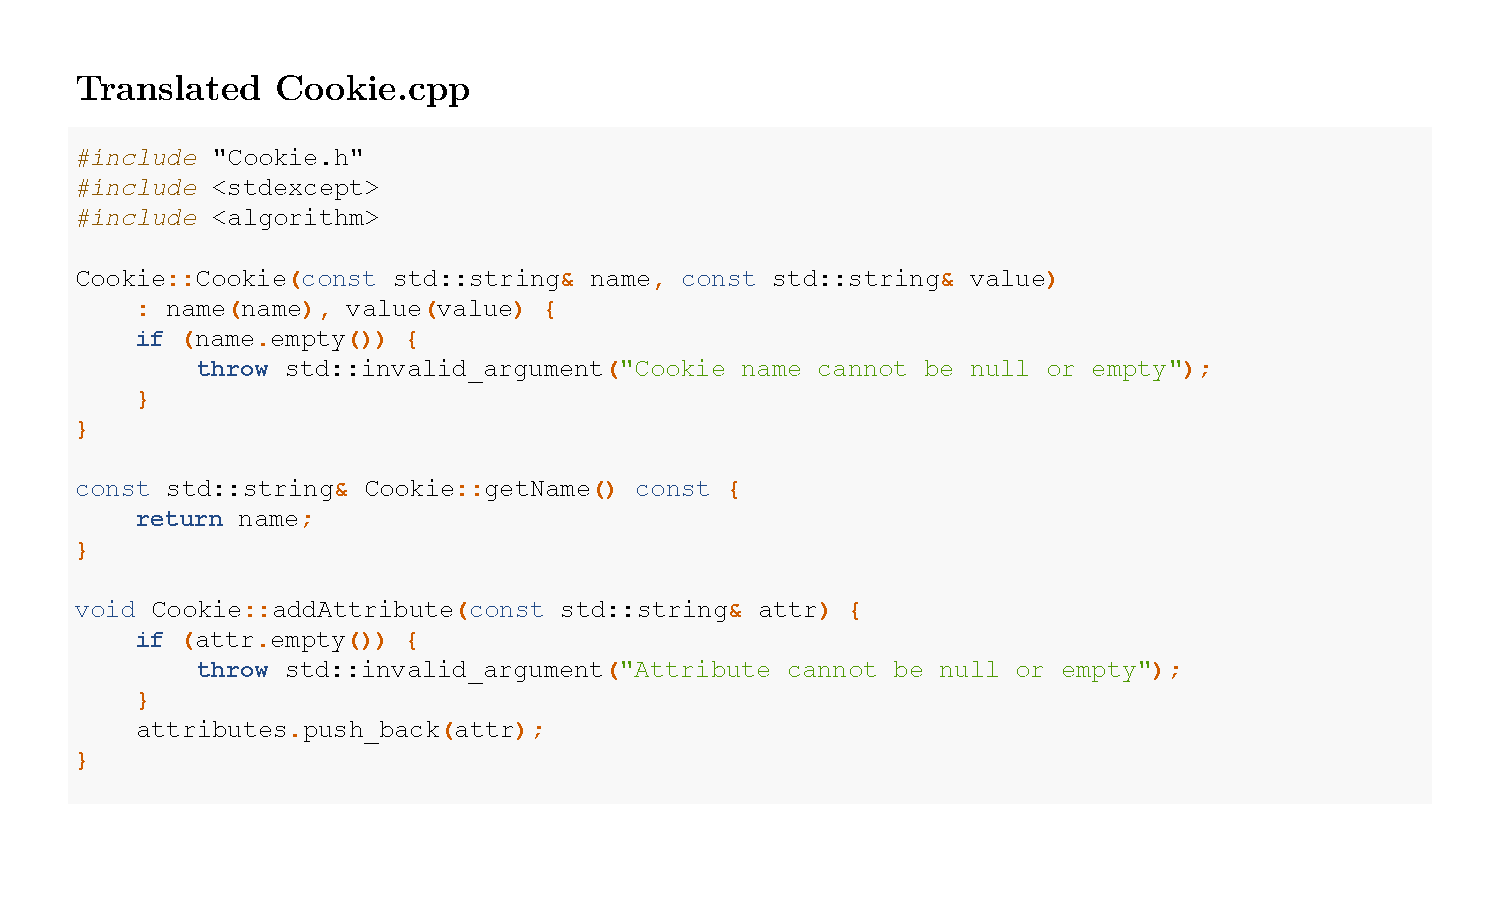
\includegraphics[width=\columnwidth]{code/fig5-4-cookie-translated-cpp.pdf}
\caption{Translated Cookie.cpp}
\label{fig:cpp-impl}
\end{figure}

\subsubsection{Compilation Agent in Action}

During initial compilation, errors are encountered and automatically resolved:

\textbf{Initial Error}:
\begin{verbatim}
Cookie.cpp:15:22: error: use of deleted function
'std::basic_string<char>::basic_string()'
\end{verbatim}

\textbf{Agent Analysis and Fix}:
\begin{figure}[h]
\centering
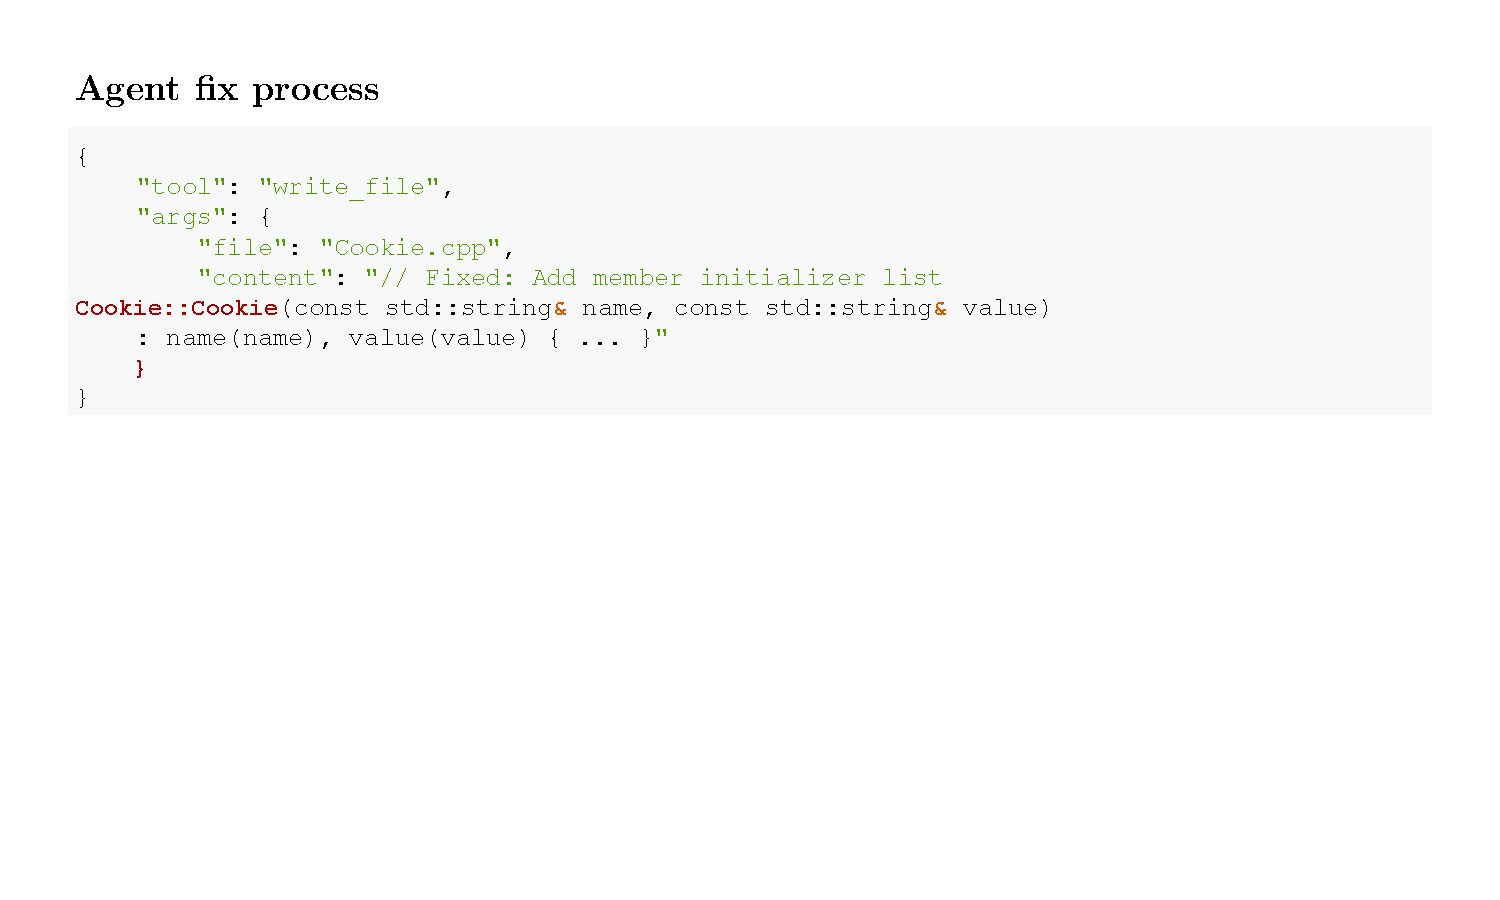
\includegraphics[width=\columnwidth]{code/fig5-5-agent-fix-process.pdf}
\caption{Agent fix process}
\label{fig:agent-fix}
\end{figure}

\subsection{Example: Generic Translation}

\subsubsection{Java Generic Class}

\begin{figure}[h]
\centering
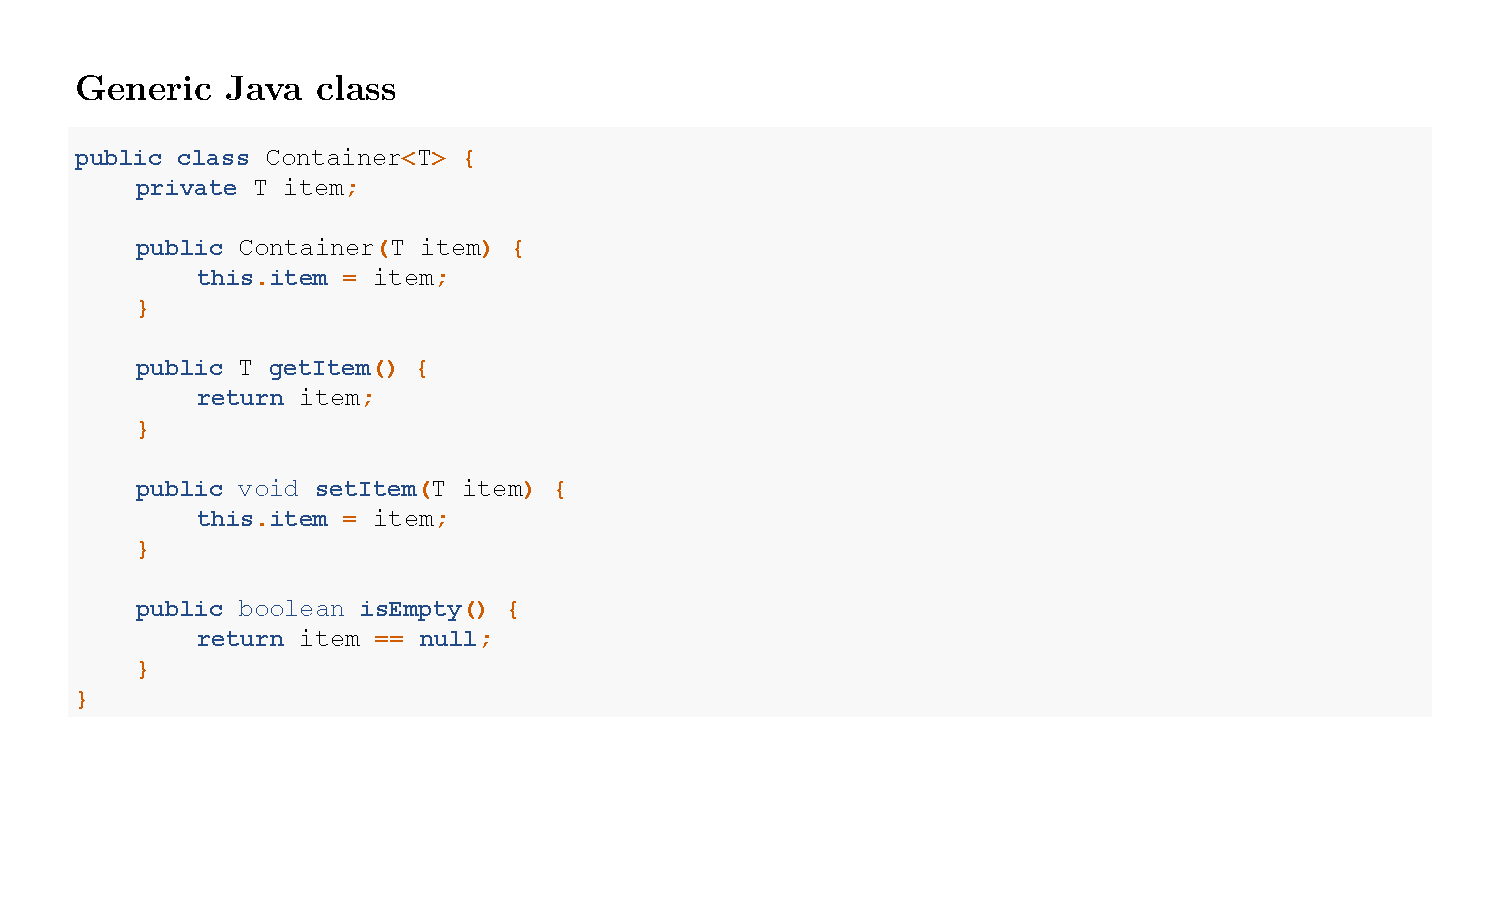
\includegraphics[width=\columnwidth]{code/fig5-6-generic-java-class.pdf}
\caption{Generic Java class}
\label{fig:java-generics}
\end{figure}

\subsubsection{C++ Template Translation}

\begin{figure}[h]
\centering
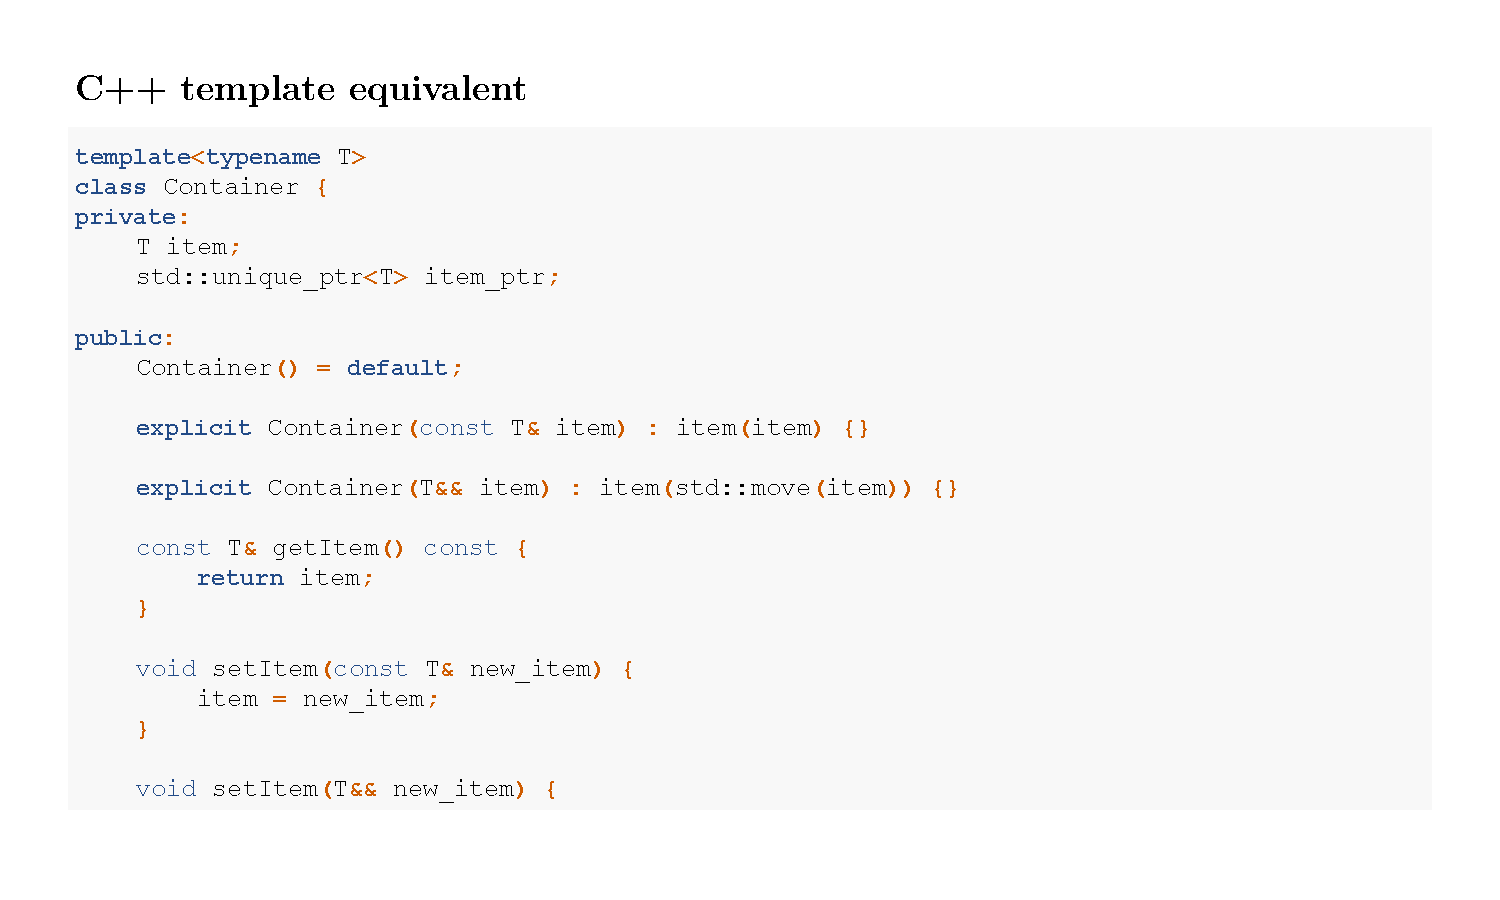
\includegraphics[width=\columnwidth]{code/fig5-7-cpp-template-equivalent.pdf}
\caption{C++ template equivalent}
\label{fig:cpp-templates}
\end{figure}

\subsection{Error Resolution Examples}

\subsubsection{Memory Management Translation}

\textbf{Problem}: Java relies on garbage collection, C++ requires explicit memory management.

\textbf{Solution Strategy}:
\begin{enumerate}
\item Replace object references with smart pointers when needed
\item Use RAII principles for resource management
\item Implement proper copy/move semantics
\end{enumerate}

\begin{figure}[h]
\centering
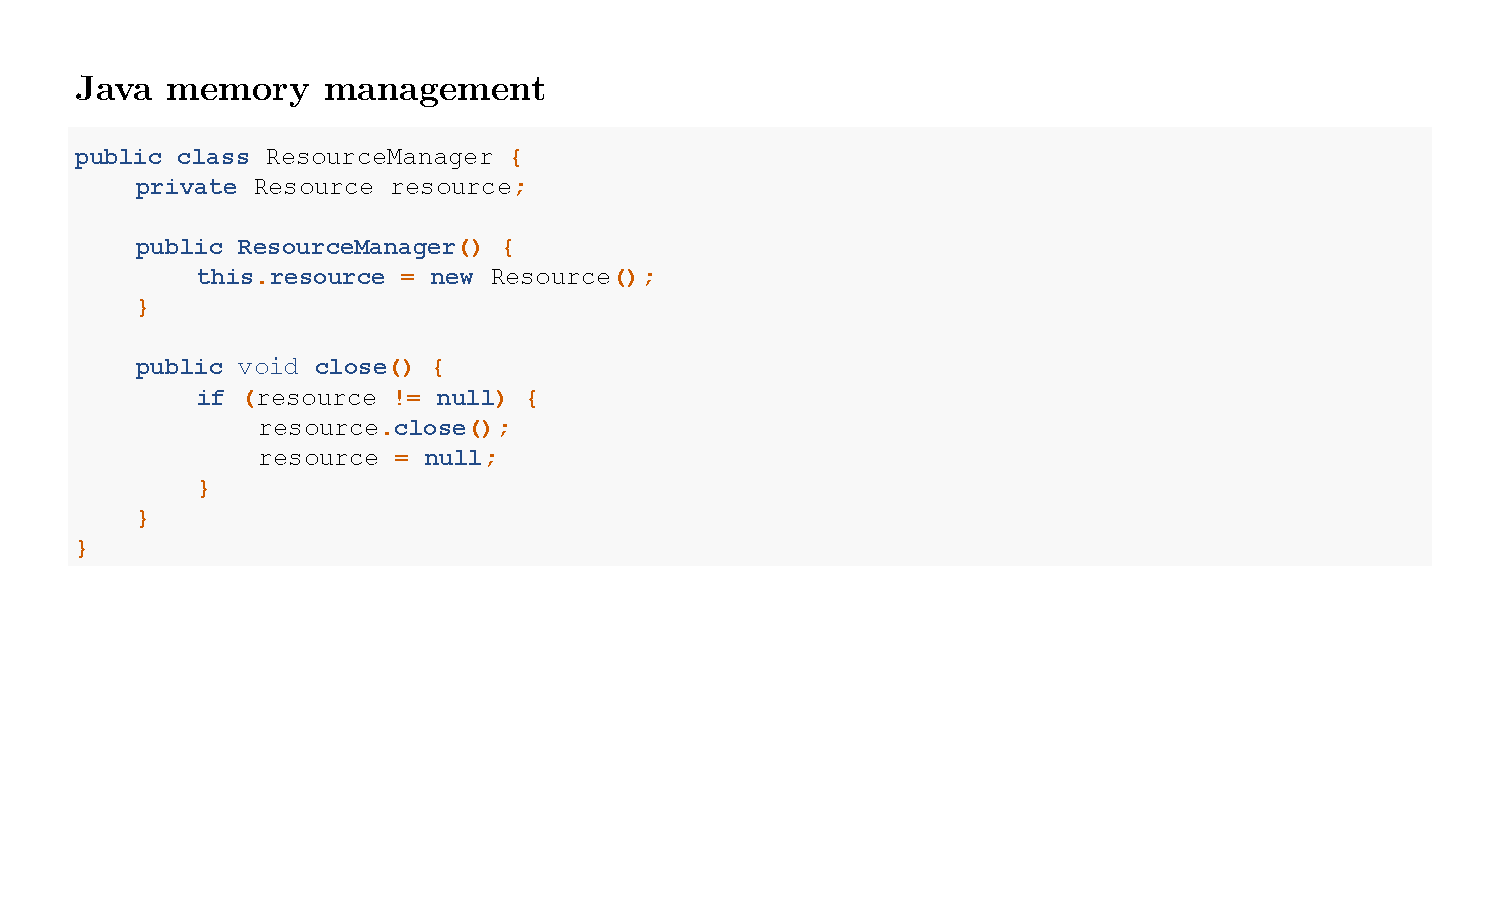
\includegraphics[width=\columnwidth]{code/fig5-8-java-memory-management.pdf}
\caption{Java memory management}
\label{fig:java-memory}
\end{figure}

\begin{figure}[h]
\centering
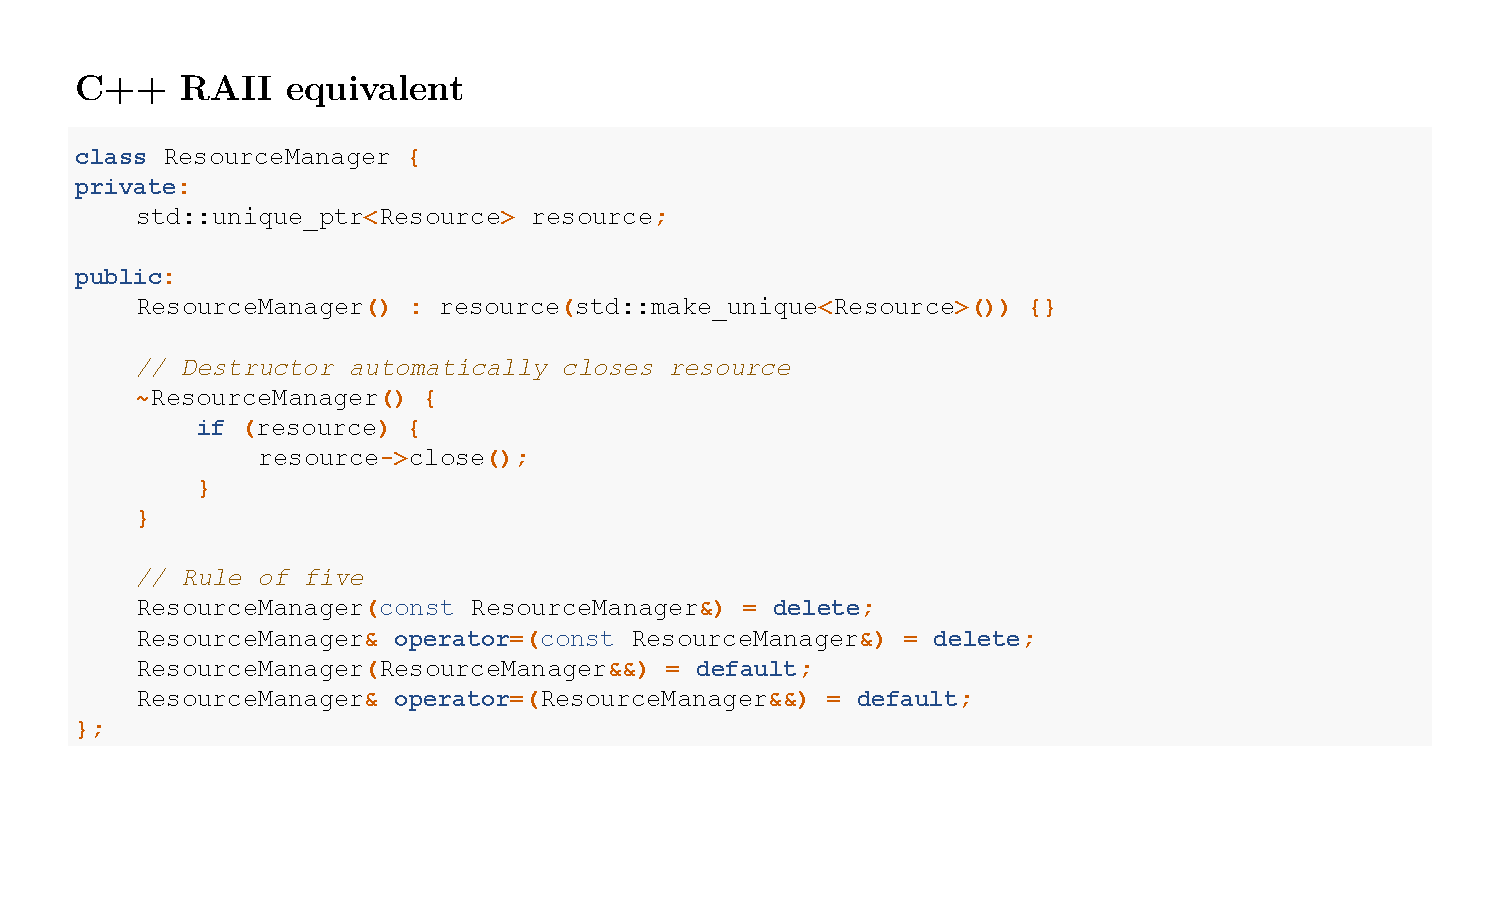
\includegraphics[width=\columnwidth]{code/fig5-9-cpp-raii-equivalent.pdf}
\caption{C++ RAII equivalent}
\label{fig:cpp-raii}
\end{figure}

\subsubsection{Exception Handling Translation}

\textbf{Problem}: Java has checked exceptions, C++ uses unchecked exceptions.

\textbf{Solution}:
\begin{itemize}
\item Map Java exceptions to appropriate C++ exceptions
\item Replace checked exception requirements with documentation
\item Use noexcept specifier where appropriate
\end{itemize}

\begin{figure}[h]
\centering
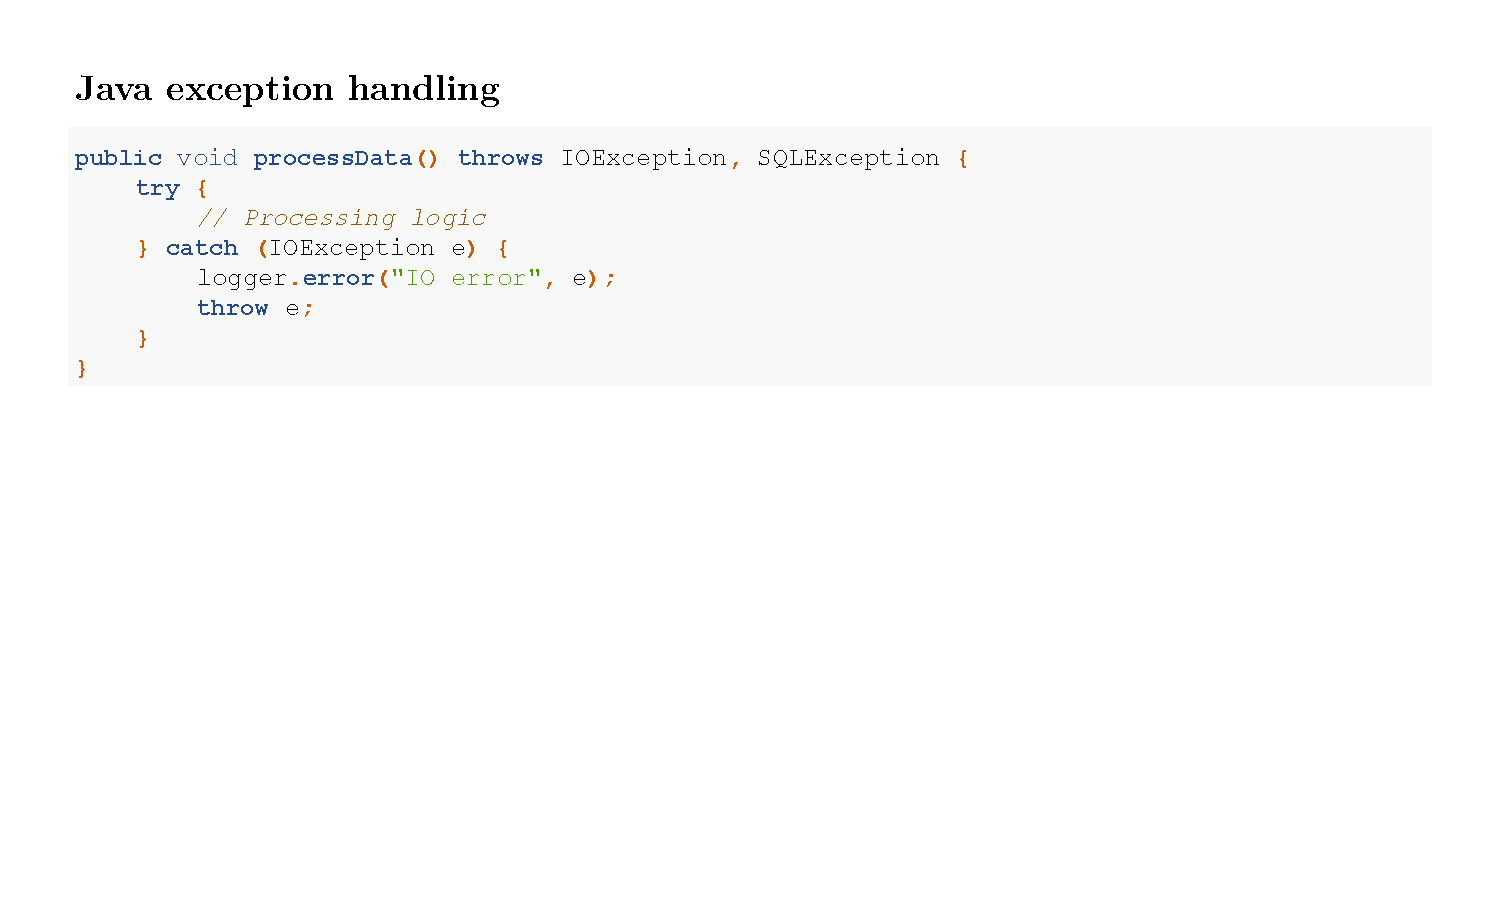
\includegraphics[width=\columnwidth]{code/fig5-10-java-exception-handling.pdf}
\caption{Java exception handling}
\label{fig:java-exceptions}
\end{figure}

\begin{figure}[h]
\centering
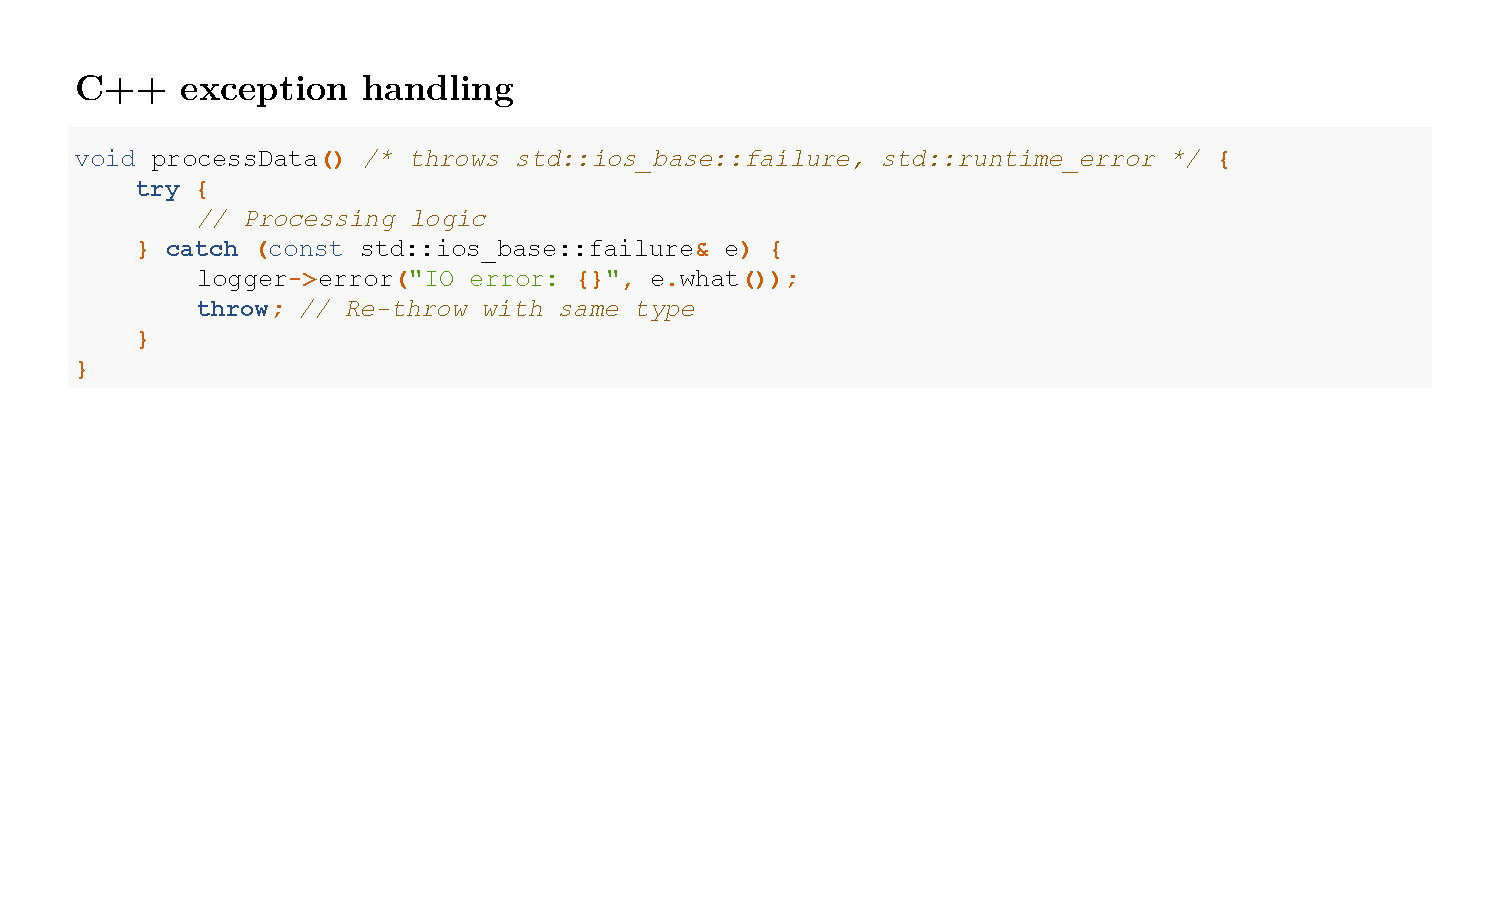
\includegraphics[width=\columnwidth]{code/fig5-11-cpp-exception-handling.pdf}
\caption{C++ exception handling}
\label{fig:cpp-exceptions}
\end{figure}

\subsection{Performance Optimization Examples}

The framework automatically identifies opportunities for C++-specific optimizations:

\subsubsection{Move Semantics}

\begin{figure}[h]
\centering
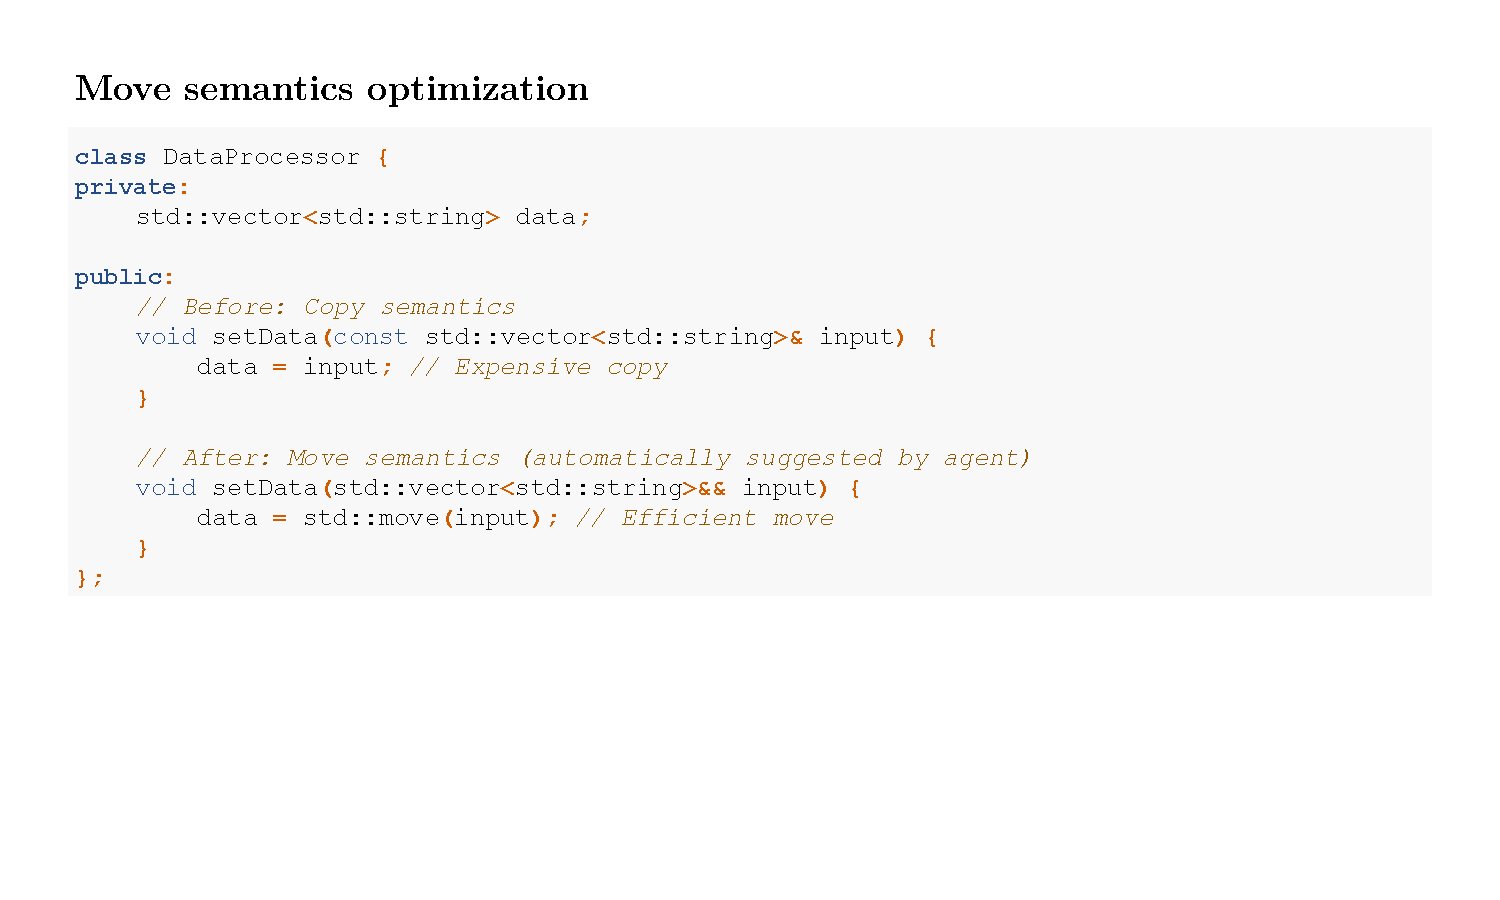
\includegraphics[width=\columnwidth]{code/fig5-12-move-semantics-optimization.pdf}
\caption{Move semantics optimization}
\label{fig:move-semantics}
\end{figure}

\subsubsection{Template Specialization}

\begin{figure}[h]
\centering
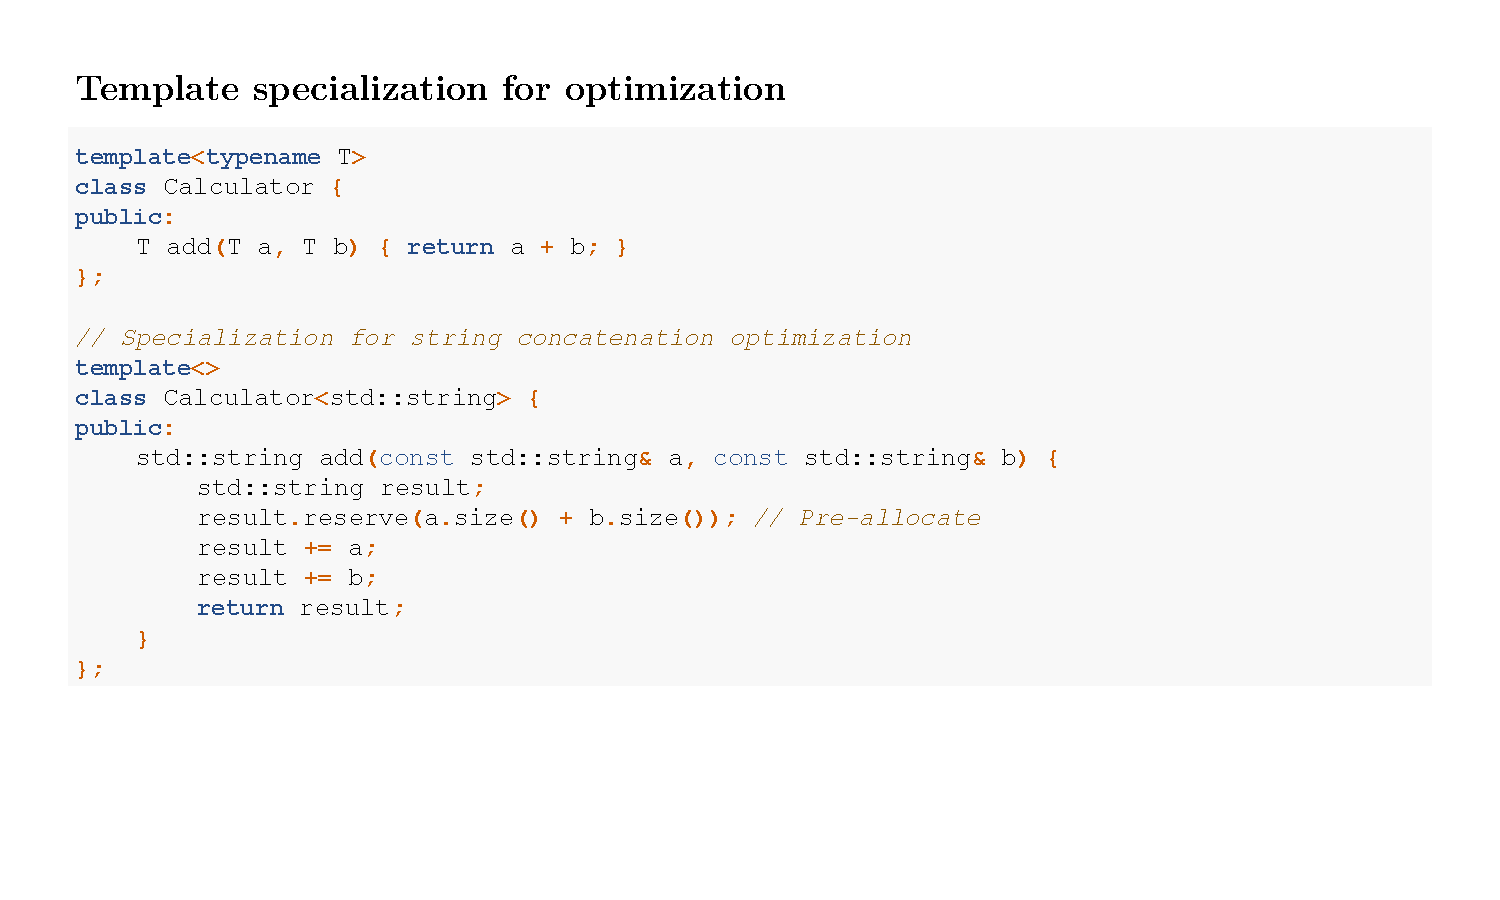
\includegraphics[width=\columnwidth]{code/fig5-13-template-specialization.pdf}
\caption{Template specialization for optimization}
\label{fig:template-specialization}
\end{figure}

\subsection{Tool Usage Statistics}

Based on our evaluation, the compilation agent's most frequently used operations:

\begin{table}[h]
\centering
\small
\begin{tabular}{lc}
\toprule
\textbf{Tool Operation} & \textbf{Usage Frequency} \\
\midrule
compile\_file & 156 times \\
read\_file & 89 times \\
write\_file & 67 times \\
create\_file & 23 times \\
\bottomrule
\end{tabular}
\caption{Compilation agent tool usage statistics}
\label{tab:tool-usage}
\end{table}

The most common error categories and their resolution strategies are:

\begin{itemize}
\item \textbf{Missing Headers}: Automatically add required include statements
\item \textbf{Type Conversion}: Apply appropriate cast operations and template parameters
\item \textbf{Namespace Issues}: Insert proper namespace declarations
\item \textbf{Link Errors}: Generate missing function implementations
\end{itemize}

\subsection{User Experience}

The tool provides comprehensive logging and progress tracking:

\begin{figure}[h]
\centering
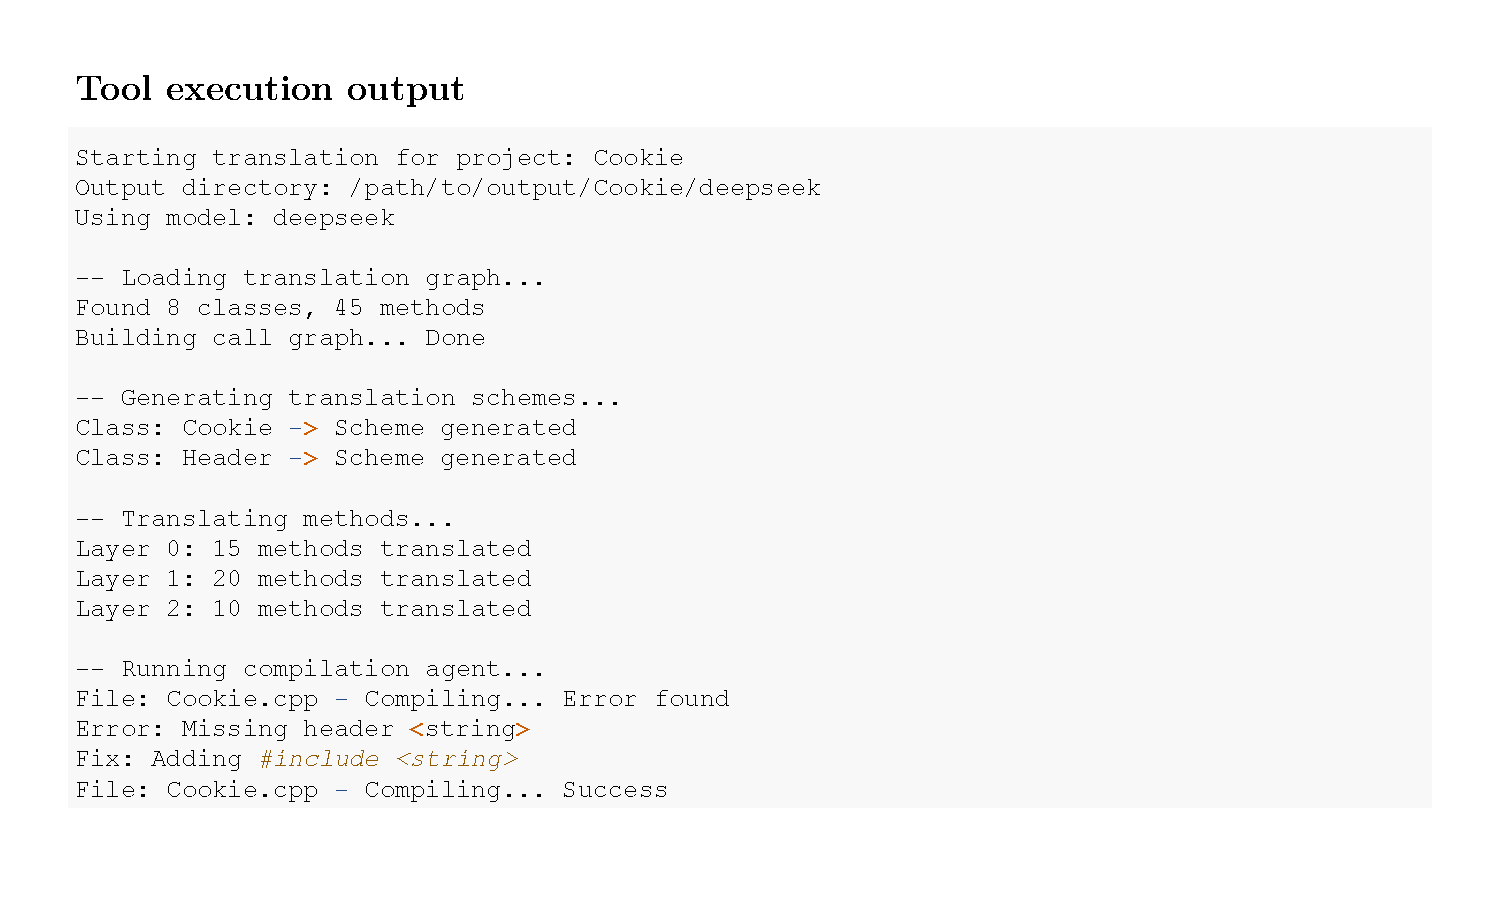
\includegraphics[width=\columnwidth]{code/fig5-14-tool-execution-output.pdf}
\caption{Tool execution output}
\label{fig:tool-output}
\end{figure}

This demonstration illustrates how \tool{} handles the complex process of Java-to-C++ translation, combining static analysis, hierarchical translation, and intelligent error recovery to produce high-quality C++ code.